\documentclass[10pt,a4paper]{article}

\usepackage[a4paper, top=0.9cm, bottom=0.9cm, left=1cm, right=1cm]{geometry}
\usepackage{graphicx}
\usepackage{float}
\usepackage{amsmath}
\usepackage{amssymb}
\usepackage{xcolor}
\usepackage{mdframed}
\usepackage{parskip}
\usepackage{enumitem}
\usepackage{titlesec}
\usepackage{booktabs}
\usepackage{array}
\usepackage{tikz}
\usetikzlibrary{arrows.meta, positioning}
\usepackage[T1]{fontenc}

\graphicspath{{../../reference/Network_extracted/figures/Lecture3/}}

\definecolor{keyblue}{RGB}{30, 80, 160}
\definecolor{keybluebg}{RGB}{220, 235, 255}
\definecolor{noteorange}{RGB}{200, 100, 0}
\definecolor{noteorangebg}{RGB}{255, 240, 215}
\definecolor{warnred}{RGB}{180, 30, 30}
\definecolor{warnredbg}{RGB}{255, 220, 220}
\definecolor{defgreen}{RGB}{20, 110, 50}
\definecolor{defgreenbg}{RGB}{215, 245, 225}
\definecolor{headernavy}{RGB}{25, 35, 90}

\newmdenv[linecolor=keyblue,backgroundcolor=keybluebg,linewidth=1.5pt,
  leftline=true,rightline=false,topline=false,bottomline=false,
  innerleftmargin=7pt,innerrightmargin=6pt,
  innertopmargin=3pt,innerbottommargin=3pt,
  skipabove=3pt,skipbelow=3pt]{keybox}

\newmdenv[linecolor=noteorange,backgroundcolor=noteorangebg,linewidth=1.5pt,
  leftline=true,rightline=false,topline=false,bottomline=false,
  innerleftmargin=7pt,innerrightmargin=6pt,
  innertopmargin=3pt,innerbottommargin=3pt,
  skipabove=3pt,skipbelow=3pt]{notebox}

\newmdenv[linecolor=defgreen,backgroundcolor=defgreenbg,linewidth=1.5pt,
  leftline=true,rightline=false,topline=false,bottomline=false,
  innerleftmargin=7pt,innerrightmargin=6pt,
  innertopmargin=3pt,innerbottommargin=3pt,
  skipabove=3pt,skipbelow=3pt]{defbox}

\newmdenv[linecolor=warnred,backgroundcolor=warnredbg,linewidth=1.5pt,
  leftline=true,rightline=false,topline=false,bottomline=false,
  innerleftmargin=7pt,innerrightmargin=6pt,
  innertopmargin=3pt,innerbottommargin=3pt,
  skipabove=3pt,skipbelow=3pt]{warnbox}

\titleformat{\section}[block]{\normalsize\bfseries\color{headernavy}}{}{0pt}{}
  [\vspace{1pt}\rule{\linewidth}{0.6pt}\vspace{2pt}]
\titleformat{\subsection}[block]{\small\bfseries\color{keyblue}}{}{0pt}{}
\titlespacing*{\section}{0pt}{5pt}{2pt}
\titlespacing*{\subsection}{0pt}{3pt}{1pt}

\setlist{nosep, topsep=1pt, itemsep=1pt, leftmargin=1.3em}
\parskip=2pt
\parindent=0pt

% ===========================================================================
\begin{document}
% ===========================================================================

\begin{center}
  {\large\bfseries\color{headernavy} Q3 \textemdash{} Clock Sync \& Impact of Clock Offset on Distributed Sensor Data}\\[1pt]
  {\small MM3 $\cdot$ Hans-Peter Schwefel}
\end{center}
\vspace{1pt}\hrule height 1pt\vspace{4pt}

% ===========================================================================
\section*{1\quad Clock Imperfections}
% ===========================================================================
Ideally every component would have a perfect clock --- 
continuous and tracking real time exactly.  
In reality every clock \textbf{drifts} from true time, and no two clocks drift at the same rate.\\[2pt]
These imperfections matter because clock offset between nodes corrupts distributed sensor averages and breaks time-based coordination.

\begin{minipage}[c]{0.44\textwidth}
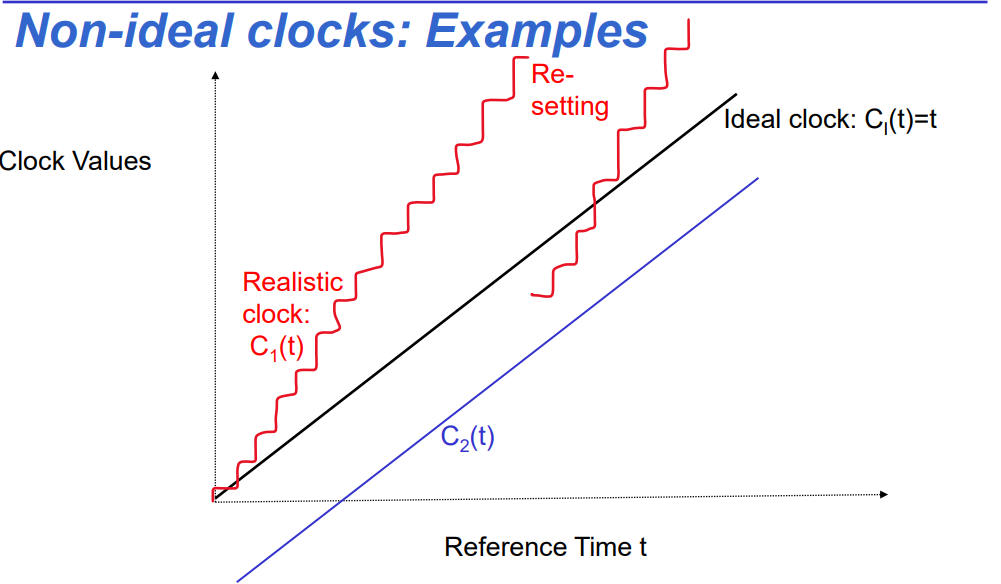
\includegraphics[width=\linewidth]{nonidealclock.png}
\end{minipage}\hfill
\begin{minipage}[c]{0.53\textwidth}
\begin{defbox}
We describe clock imperfections by two factors: 
\begin{itemize}
  \item \textbf{Granularity} $g$: (how often the clock updates)
  \item \textbf{drift rate} (how fast it deviates from real time)
\end{itemize}
Each clock has its own maximum drift rate $\rho_k$ (Tolerance). 
\[ \left|\frac{dC_k(t)}{dt} - 1\right| \leq \rho_k \]
\end{defbox}
\begin{notebox}
  \textbf{Don't know if keep yet} Modelled as cont.\ differentiable functions.
\end{notebox}
\vspace{2pt}
\begin{keybox}
Importance Measures are: \\
\textbf{Precision} $\pi$: $|C_i(t) - C_k(t)| \leq \pi$ \quad (two local clocks)\\[2pt]
\textbf{Accuracy} $\alpha$: $|C_k(t) - t| \leq \alpha$ \quad (vs.\ UTC ref)
\end{keybox}
\end{minipage}
\vspace{6pt}
\\Because of drift, clocks must be periodically re-synced --- 
otherwise they diverge from real time \\ and from each other indefinitely in distributed systems. \\[4pt]

% ===========================================================================
\section*{2\quad Sync Protocols: Cristian's $\to$ Berkeley $\to$ NTP}
% ===========================================================================
\textbf{Goal in distributed:} all clocks agree $\Rightarrow$ minimise precision. \\[6pt]
Sync protocols fall into two types:
\begin{itemize}
  \item \textbf{internal} --- clocks agree with each other (minimise precision, no external reference needed)
  \item \textbf{external} --- clocks sync to a universal reference such as UTC (minimise accuracy).
\end{itemize} \vspace{0.5em}
We go from simplest to most sophisticated: \\
\begin{minipage}[t]{0.38\textwidth}
\subsection*{Cristian's Protocol}
Gives the basic idea but has real-world problems;
\begin{enumerate}
  \item Client sends request
  \item Server replies: $t_B = C_B(t)$
  \item Client measures RTT: $\hat{R}$
  \item $C_A \leftarrow t_B + \hat{R}/2$ \; (precision $= \hat{R}/2$)
\end{enumerate}
\begin{warnbox}
\textbf{Problems:}
\begin{itemize}
\item Asymm.\ links,
\item proc.\ delays,
\item jitter $\Rightarrow$ $\hat{R}/2$ only estimate.
\end{itemize} 
\end{warnbox}
\vspace{3pt}
\subsection*{Berkeley (improves Cristian's)}
\begin{enumerate}
  \item Master polls all slaves
  \item Collects clock values
  \item Estimates RTTs; removes outliers
  \item Computes avg.\ time
  \item Sends adjustments to slaves
\end{enumerate}
\begin{keybox}
Berkeley Introduces Filtering of outliers\\
and polls all slaves, meaning \\
More data points $\Rightarrow$  better estimate.
\end{keybox}
\begin{notebox}
\small Master averages --- no external UTC ref needed.
\end{notebox}
\end{minipage}\hfill
\begin{minipage}[t]{0.59\textwidth}
\subsection*{NTP --- Sync to UTC via strata}
NTP scales this to the internet with UTC as the reference.
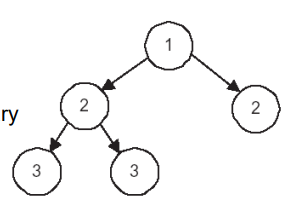
\includegraphics[width=0.5\linewidth]{stratum.png}
\begin{keybox}
\small\textbf{Clever:} 
\begin{itemize}
  \item syncs repeatedly;
  \item keeps offset/delay history;
  \item filters noisy stats;
  \item picks most reliable server (lowest variance).
\end{itemize}  
Calculate like this:
\[
\text{RTT} = (t_4 - t_1) - (t_3 - t_2)
\]
\[
\text{offset} = \tfrac{(t_2-t_1)+(t_3-t_4)}{2}
\]
Where \textbf{Timestamps:} are:
\begin{itemize}
  \item $t_1$ client send
  \item $t_2$ server rcv
  \item $t_3$ server send
  \item $t_4$ client rcv.
\end{itemize}
\end{keybox}
\end{minipage}

\clearpage
\section*{3\quad Impact of Clock Offset on Sensor Data}
% ===========================================================================
When distributed sensors assume clocks are synchronised and average over the same timestep (e.g.\ power consumption),\\
a clock offset $\delta$ causes them to physically sample \textbf{different time intervals} --- corrupting the shared average.
\vspace{3pt}

\begin{minipage}[c]{0.50\textwidth}
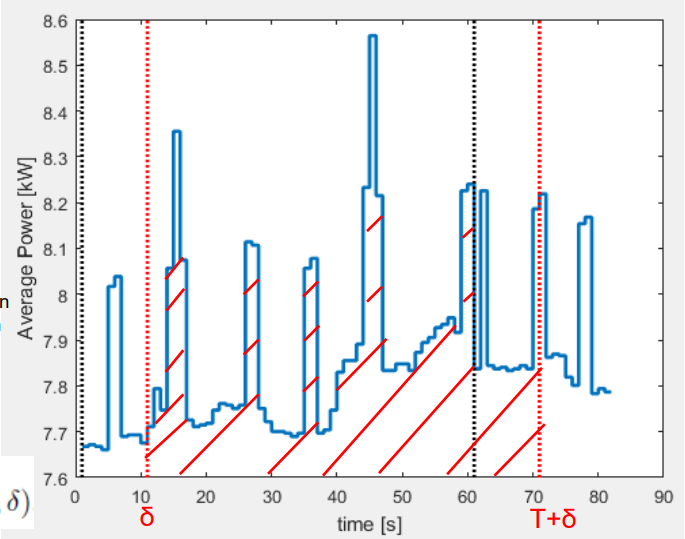
\includegraphics[width=\linewidth]{delayedtimeperiod.png}
\end{minipage}\hfill
\begin{minipage}[c]{0.47\textwidth}
\begin{defbox}
 Even a small offset $\delta$ shifts the integration window 
\begin{itemize}
  \item two sensors integrating over period $T$
  \item averaging over physically different intervals
  \item results can differ significantly
\end{itemize} (e.g.\ $\delta{=}12$\,ms already visible in figure). \\[4pt]
\textbf{Reference interval:} $[0,\,T]$\\[2pt]
\textbf{Offset interval:} $[\delta,\,T{+}\delta]$\\[3pt]
Both claim same window but physically differ by $\delta$.\\[3pt]
\textbf{Measured avg.:}
\[ \hat{M}(T,\delta) := \frac{1}{T}\int_{\delta}^{T+\delta} M(t)\,dt \]
\textbf{Meas.\ deviation:}
\[ \varepsilon(T,\delta) := \hat{M}(T,0) - \hat{M}(T,\delta) \]
\end{defbox}
\vspace{3pt}
\begin{warnbox}
\small Devices have 0.1--1\% error, but \emph{assuming} sync'd clocks is what causes the real problem --- offset introduces systematic bias in averaged sensor data.
\end{warnbox}
\end{minipage}

\vspace{4pt}
% ===========================================================================
\section*{4\quad Markov Modulated Process}
% ===========================================================================

To analytically compute the measurement deviation $\varepsilon(T,\delta)$ from Section 3, we need a model for the sensor signal $M(t)$. Real signals like power consumption don't vary randomly --- they switch between a few \textbf{device states} (e.g.\ idle, active, transmitting) that evolve as a CTMC.

The \textbf{Markov Modulated Process} extends a CTMC by attaching an emission value to each state --- giving a tractable stochastic model for $M(t)$.

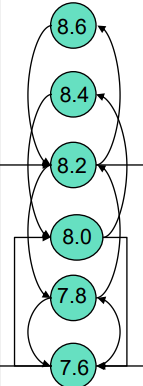
\includegraphics[width=0.2\linewidth, angle=90]{markovmodulated.png}
\begin{keybox}
\small Extends CTMC by attaching a \textbf{value} (e.g.\ power) at each state. Discretise continuous meas.\ values to states.\\[4pt]
State distribution:
\[ \underline{P}(t) = \underline{P}(0)\exp(Qt) \]
Power emission matrix ($E_{ii}$ = power in state $i$):
\[ E = \mathrm{diag}(e_1, e_2, \ldots, e_n) \]
\end{keybox}

% ===========================================================================
\section*{5\quad Expected Power \& Steady-State}
% ===========================================================================

\begin{minipage}[t]{0.48\textwidth}
\begin{keybox}
\small\textbf{Steady-state distribution} $\underline{\pi}$: solve $\underline{\pi} Q = \underline{0}$, $\sum_i \pi_i = 1$.\\[3pt]
\textbf{Expected power:}
\[ \bar{P} = \underline{\pi} \cdot \underline{e} = \sum_i \pi_i \, e_i \]
where $e_i = E_{ii}$ is power in state $i$.\\[3pt]
For time-varying: $\underline{P}(t)E\,\underline{1}^T$ gives instantaneous expected power.
\end{keybox}
\end{minipage}\hfill
\begin{minipage}[t]{0.48\textwidth}
\begin{notebox}
\small\textbf{Clock precision $\Rightarrow$ meas.\ error bound:}\\
If precision is $\pi$ (two clocks differ by at most $\pi$), then offset $\delta \leq \pi$. The measurement deviation $\varepsilon(T,\delta)$ is bounded by the signal's max rate of change times $\delta$.\\[3pt]
Tight clock sync $\Rightarrow$ small $\delta$ $\Rightarrow$ small $\varepsilon$ $\Rightarrow$ valid power comparison across nodes.
\end{notebox}
\vspace{3pt}
\begin{defbox}
\small\textbf{Perfect vs.\ offset period:}\\
$[0,T]$ vs.\ $[\delta, T{+}\delta]$ --- overlap $= T{-}\delta$. If $\delta \ll T$ the bias is small; if $\delta \approx T$ the windows barely overlap.
\end{defbox}
\end{minipage}

\vspace{4pt}

\clearpage
% ===========================================================================
\section{Extra shit dont take into exam}
\section*{6\quad Two Methods for Loss Estimation}
% ===========================================================================

\begin{minipage}[t]{0.48\textwidth}
\subsection*{$L_1$: Total Loss (Energy Balance)}
\[
L_1 = T\!\cdot\!\left(P_\mathrm{imp}^{(0)} - P_\mathrm{exp}^{(0)} + \sum_{j=1}^{K}\!\left(P_\mathrm{inj}^{(j)} - P_\mathrm{cons}^{(j)}\right)\right)
\]
\begin{warnbox}
\small\textbf{Extremely sensitive to $\delta$:} subtracts readings from \emph{different devices}. Loss is a \emph{small difference of large numbers}.\\[2pt]
$206\!-\!200=6\,\text{kW}$ true loss; $\delta=8\,\text{s}$ (machine switches on) $\Rightarrow$ one meter reads 205\,kW $\Rightarrow$ computed $=1\,\text{kW}$. \textbf{83\% error.}
\end{warnbox}
\end{minipage}\hfill
\begin{minipage}[t]{0.48\textwidth}
\subsection*{$L_2$: Technical Loss (Ohmic Heating)}
\[
L_2 = T\cdot\sum_{j=1}^{C} I_j^2\, R_j
\]
\begin{keybox}
\small\textbf{Robust to $\delta$:} each $I_j^2 R_j$ term comes from a \emph{single sensor} on one cable segment --- no cross-device subtraction. Cable current is an aggregate of many loads $\Rightarrow$ changes slowly $\Rightarrow$ edge-slice error $\varepsilon$ stays small.
\end{keybox}
\end{minipage}

\vspace{3pt}

\begin{minipage}[c]{0.52\textwidth}
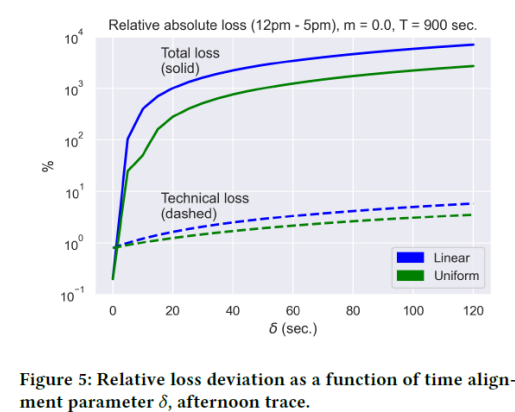
\includegraphics[width=\linewidth]{L1vsL2.png}
\end{minipage}\hfill
\begin{minipage}[c]{0.45\textwidth}
\begin{notebox}
\small\textbf{Key result} (log-scale, $T=900\,\text{s}$, afternoon):
\begin{itemize}
  \item $L_1$ (solid): error reaches \textbf{thousands \%} by $\delta\!\sim\!120\,\text{s}$
  \item $L_2$ (dashed): saturates $\approx\!10\%$ --- $I^2$ changes smoothly
\end{itemize}
\textbf{Bottom line:} for NTP-synced devices ($\delta\sim$ms--s) $L_1$ may be ok; after reboot/GPS loss ($\delta\sim30$--120\,s) $L_1$ is useless. Use $L_2$ when clocks may drift.
\end{notebox}
\end{minipage}

\end{document}
